\section{AI in Fault Detection}
A software fault (also called bug) refers to a static defect in the software. When the software is executed with a certain input, a software fault may result in an incorrect internal state, which is referred to as software error. If the software error is propogated to the output of the software, and results in incorrect behaviors with respect to the requirements or other description of the expected behavior, a software failure occurs~\cite{testbook}. 

As the size of complexity of software has grown quickly in past decades, the difficulty of finding and fixng software faults has increased. Among the different types of faults, concurrency faults are the most notorious, due to their non-deterministic nature. Concurrency faults depend not only on inputs and execution environments, but also on threadinterleaving and other timing-related events that are to be manifested, which creates challenges to expose and detect concurrency faults during in-house testing. With the pervasiveness of multi-core machines and concurrent programs, this problem is becoming more and more severe.

Besides concurrency faults, semantic faults are another form of hard-to-detect faults. Typical semantic faults are caused by missing the reassignment of some variables or incorrectly reuse some variables. Such faults are program-specific and difficult to detect by using only in-housing testing. Finally, memory corruption faults such as buffer overflow and dangling pointer are also important, since they can be exploited by malicious users.

To automatically identify such faults, Shi et al.~\cite{wrongDefinition} proposes an approach to first learn the Definition-Use Invariants and then use the learned knowledge of Definition-Use for detecting faults. They observed that regardless of the difference between these faults' root causes, many of them share a common characteristic: when triggered, they usually are followed by an incorrect data flow, i.e., a read instruction uses the value from an unexpected definition, referred to as an incorrect definition. Such commonality indicates that, if we can detect such incorrect definition-use data flow, it is possible to identify these faults automatically, regardless of their different root causes.

Their approach leverages in-house testing as training runs to extract the definition-use invariants. To tolerate insufficient training, their approach automatically prunes out unlikely invariants and violations, and ranks remaining violations based on confidence. Their approach also considers possible training noises (which
may be incorrectly labeled training runs).

\subsection{Definition-Use Invariants}
\textbf{Local/Remote (LR) Invariants.} In concurrent programs, certain read instructions may use only local definitions or only remote definitions (maybe for the purpose of communication or synchronization). LR invariants can be used to describe these properties. Formally speaking, an LR invariant, $LR(r)$, at a read instruction, $r$, equals to “LOCAL” (respectively “REMOTE”) if $r$ uses only definitions from the local (respectively remote) thread. Such invariants are denoted as LR-Local and LR-Remote, respectively. If $r$ can read from either a local or a remote definition, $r$ has no LR invariant. Figure \ref{fig:invariants}(a) illustrates the basic idea of LR invariant.

\begin{figure}
\centering
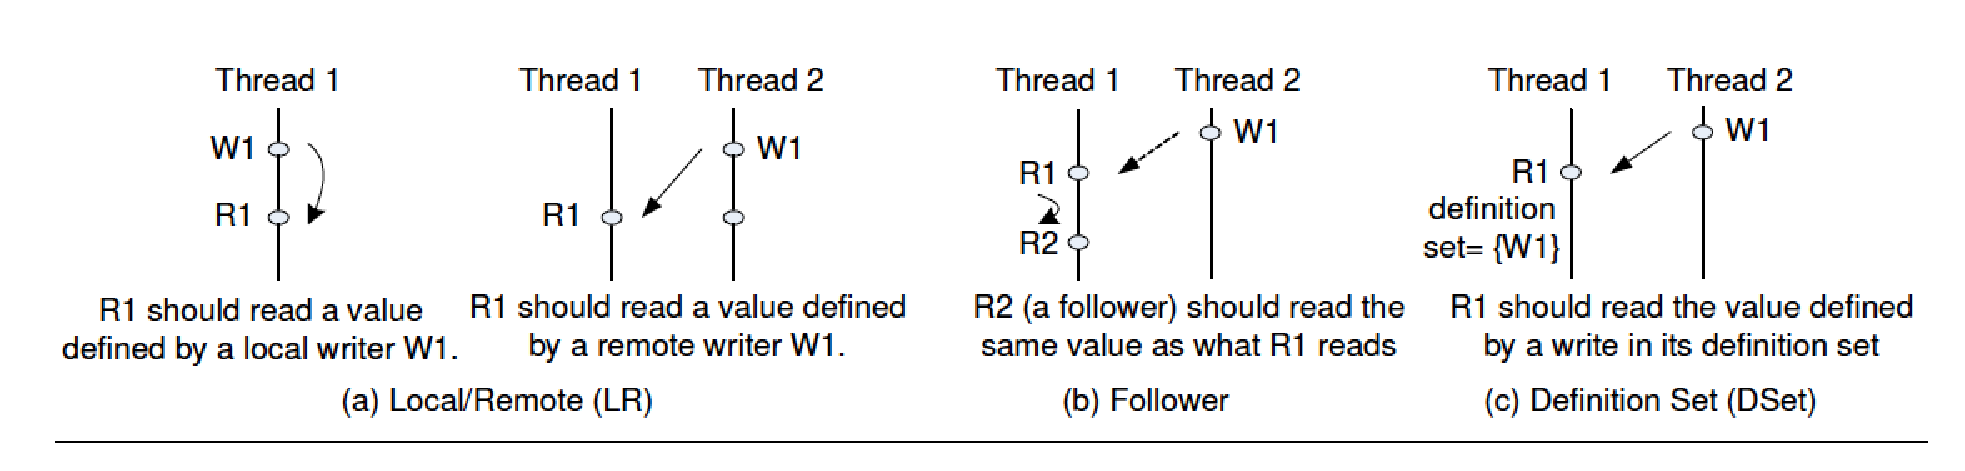
\includegraphics[scale=0.5,clip]{fig/invariants.eps} 
\caption{\label{fig:invariants}Examples of real-world definition-use invariants and their violations.} 
\end{figure}

\textbf{Follower Invariants.} In concurrent programs, developers tend to make assumptions about the atomicity of certain code regions. The LR invariants already captures the case of read-after-write data flow relation in an assumed atomic region, but not the read-after-read case, which can be captured by using a Follower Invariant. Specifically, for two consecutive reads, $r1$ and $r2$, to the same location from the same thread, if $r2$ always uses the same definition as $r1$, $r2$ has a Follower invariant. Follower is different from LR because as long as $r2$ uses the same definition as $r1$, the definition can come from either local or remote. Figure \ref{fig:invariants}(b) demonstrates Follower invariants.

\textbf{Definition Set (DSet) Invariants.} Although concurrent programs have special inter-thread data flows, definition-use is not specific to only concurrent programs. Definition Set (DSet) invariant is suitable for identify faults in both sequential and concurrent programs. A DSet invariant at a read instruction is defined as the set of all write instructions whose definitions this read instruction may use. Figure \ref{fig:invariants}(c) shows a DSet invariant at $R1$. Every read instruction has such a DSet. When an instruction violates a DSet invariant by consuming a value defined by an instruction outside its DSet, this instruction may indicate a likely fault.


\subsection{Invariant Extraction}
To identify faults using definition-use invariants, their approach consists of two phases: (1) an extraction phase for inferring definition-use invariants; and (2) a detection phase for detecting invariant violations and reporting potential faults after pruning and ranking. Figure \ref{fig:overview} shows the overview of their approach.

\begin{figure}[b]
\centering
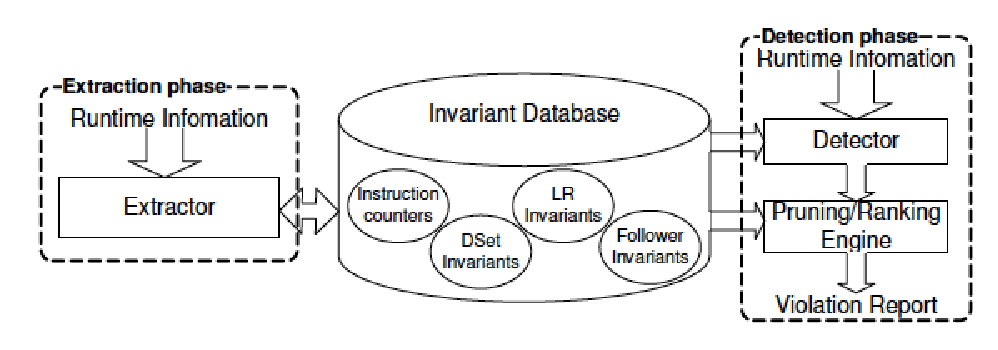
\includegraphics[scale=0.6,clip]{fig/overview.eps} 
\caption{\label{fig:overview}Overview of fault detection using definition-use invariants.} 
\end{figure}

\textbf{DSet invariant extraction}. Their approach obtains DSet by collecting all definitions that are used
by $I_U$ (read instruction) during training runs. For each memory location, their approach stores its most recent $I_D$ (write instruction) in a global hash-table, called Definition-Table. At a read instruction $i_u$, their approach retrieves its definition id from the Definition-Table and uses id's corresponding static instruction ID to update $I_U$'s DSet:

$$ DSet(I_U) \leftarrow DSet(I_U) \bigcup \{I_D\}$$

After the training phase, information for every instructions' DSet is stored into the invariant database along with some statistical information such as the number of times $I_U$ and $I_D$ are executed, and so on. Such statistical information is used for the purpose of pruning and ranking in later phases.

\textbf{LR invariant extraction.} In order to infer LR invariants, their approach first obtains the knowledge of which thread provides the definition for a read instruction by using the Definition-Table. In particular, when $i_u$ is executed, their approach identifies its definition id from the Definition-Table. Their approach then compares the thread identifiers, $T(iu)$ and $T(id)$, to determine whether they are from the same thread or not. Finally, their approach compares the answer with the LR($I_U$) associated with $I_U$. If they are different, LR($I_U$) is set to NO INV to indicate that there is no LR invariant at $I_U$ and this read instruction is no longer monitored for LR invariant extraction. LR($I_U$) is initialized based on the
definition source (either REMOTE or LOCAL) on the first time $I_U$ is executed. This process can be formalized as follows:

\[
LR(I_U) \leftarrow 
\begin{cases}
LOCAL, \text{if } LR(I_U) = LOCAL \wedge T(i_d) = T(i_u)\\
REMOTE, \text{if } LR(I_U) = REMOTE \wedge T(i_d) <> T(i_u)\\
NO\_INV, \text{Otherwise } 
\end{cases}
\]

\textbf{Follower invariant extraction.} To infer Follower invariants, their approach stores its recent access history to determine whether an instruction and its predecessor use the same definition. Their approach maintains a bitvector for every memory location $m$, called has $read(m)$. A bit in the vector has $read(m,t)$ indicates whether the current definition to memory location $m$ has already been used by thread $t$. By checking this bit-vector before every read instruction $i_u$, their approach can easily determine whether $i_u$
and its predecessor use the same definition.

In particular, bit-vector has $read(m)$ is initialized as zero. Every write to $m$ sets all bits of $has\_read(m)$ to zero. After any read from $m$ in thread $t$, $has\_read(m, t)$ is set to one. Before executing a read instruction $i_u$, their approach checks if the corresponding bit (i.e., $has\_read(m,t)$) is one. If it is, it means that there is no new definition since thread $T(i_u)$'s last use to $m$. In other words, $i_u$ shares
the same definition with its predecessor.

To maintain and update the Follower invariant information for $I_U$, their approach associates Follower($I_U$ ) with it. This flag is set to $TRUE$ if $I_U$'s dynamic instances always share definition with their predecessors. Whenever a dynamic instance of $I_U$ uses a different definition from its predecessor, the flag is set to $FALSE$ and $I_U$ is no longer monitored for Follower invariant extraction.

$$ Follower(I_U) \leftarrow Follower(I_U) \wedge has\_read(m,T(i_u))$$


\subsection{Fault Detection}
To detect DSet invariant violation, their approach maintains a Definition-Table at runtime so that it knows which instruction provides a definition for each use. If the definition for a use is not in this use's DSet, a violation is issued. Formally speaking, the violation condition is:
$$I_D \notin DSet(I_U)$$

Detecting violations against LR invariants is also straightforward. At a monitored read, their approach checks whether this read has an LR invariant or not. If it does, their approach examines whether the monitored read and its definition come from the same thread and matches the monitored condition with the type of LR invariant (LOCAL and REMOTE) extracted at this read instruction. 
$$\{LR(I_U) = LOCAL \wedge T(i_d) <> T(i_u)\} \vee \{LR(I_U) = REMOTE \wedge T(i_d) = T(i_u)\}$$

To detect violations to Follower invariants, their appraoch checks whether an instruction with a Follower invariant shares the same definition with its predecessor (by leveraging the has $read(m)$ vector similar to that used in extraction). If not, a violation will be reported.
$$Follower(I_U) \wedge \overline{has\_read(m,T(i_u))}$$

\subsection{Pruning and Ranking}
\textbf{Pruning.} Their approach automatically prunes the following cases: (1) \textit{Barely exercised uses}: For read instructions that are never covered during training, their approach do not report any violations since their approach do not extract any invariants associated with them; (2) \textit{Barely exercised definitions}: For definitions that are never exercised during training runs, their approach also prunes them; (3) \textit{Popular uses}: Some uses, such as those in a small function called from multiple call-sites, are very popular and have a large definition set. In this case, their approach also prunes it as it might be perfectly acceptable to have yet another definition for this use during detection runs.

\textbf{Ranking.} After pruning the above cases, their ranks every unpruned violations based on its confidence. Their approach relies on the following conditions to increase the confidence of a fault: (1) many dynamic instances of the definition ($\#I_D$) and the use ($\#I_U$) during training; (2) no significant difference between the number of instances of the definition and instances of the use ($|\#ID - \#IU|$) during training; (3) small definition set ($|DSet(I_U)|$); (4) few instances of this violation pair ($\#violation_{DSet}(I_D, I_U)$) during detection.

For violations to DSet invariants, their approach computes the confidence using the following formula:
$$conf_{DSet} = \frac{\#I_D \times \#I_U}{(|\#ID - \#IU| \times |DSet(I_U)| \times \#violation_{DSet}(I_D, I_U))}$$

For LR and Follower violations, the confidence is computed based only on the number of dynamic instances of a
use during training and the number of violations occurring during detection, as follows:
$$conf_{LR}=\#I_U / \#violation_{LR}(I_U)$$
$$conf_{F}=\#I_U / \#violation_{F}(I_U)$$

\subsection{Conclusion}
Shi et al.~\cite{wrongDefinition} proposed definition-use invariants which can be used to detect a wide range of software faults, including both concurrency bugs (atomicity and order violations) and sequential bugs (memory corruptions and certain semantic faults). Their experimental results with 16 real-world applications and 20 real-world faults of different types have shown that their approach was effective in detecting 19 of them, including 2 new faults that were never reported before, while introducing only 0-3 false positives. Their training sensitivity experiments showed that their approach can reasonably tolerate insufficient training, especially with confidence-based pruning.

% Recent research works~\cite{wrongDefinition,online} that use AI techniques have advanced the research in reducing the human efforts on fault detection: Shi et al.~\cite{wrongDefinition} proposes an approach to first learn the Definition-Use Invariants and then use the learned knowledge of Definition-Use for detecting concurrency and sequential bugs; Baah et al~\cite{online} and proposes a new machine-learning technique that performs fault detection for deployed software. I plan to study in details how these research works adopt the concepts and techniques of AI to assist the task of fault detection.